% !TEX root = main.tex
\chapter{The standard model of particle physics}
\label{chap:SM}

In the following chapter the fundamental particles and forces of the standard model of particle physics are described.
Following Refs.~\cite{Griffiths:111880} and \cite{Peskin:257493} first an overview of the elementary particles is given. Following the
discrete symmetries of the \ac{SM} are described. Last the outstanding coupling of the weak interaction which is described
by the so called CKM matrix is presented.

\section{Fundamental particles and forces}
\label{sec:fundamentalparts}

The \ac{SM} is a relativistic quantum field theory. Particles are produced and destroyed via fields $\phi(x)$and the dynamics
is described through Lagrangians $\mathcal{L}\left(\phi(x),\partial_{\mu}\phi(x)\right)$. In total 12 fundamental particles
with halfinteger spin called fermions exist: six quarks and six leptons. Furthermore particles with integer spin are called
bosons. All matter is built out of fermions, while the bosons act as mediators of the forces in the \ac{SM} (see
Fig.~\cref{fig:SMparts}).

Either the quarks as the leptons are classified in three families, where each family consistes of a duplet. The quarks are further
classified into Up- and Down-type quarks. The Up-type quarks are the up- (\uquark), charm- (\cquark) and top-quark (\tquark),
and have an electrical charge of $+\frac{2}{3}e$, the Down-type quarks are the down- (\dquark), strange- (\squark) and bottom-quark
(\bquark) and carry an electrical charge of $-\frac{1}{3}e$.

In the leptonic sector particles are divided into the charged and uncharged leptons. The charged leptons are the electron (\electron),
the muon (\muon) and the \tauon (\tauon), the uncharged particles are the correspondig neutrinos (\neue, \neum, \neut). All described
fermions have an antiparticle with opposite charge. In the quarksector this differentation is also denoted  flavour.

As mentioned before particles with integer spin are called bosons. The so called gauge bosons are directly associated with the fundamental
forces in the \ac{SM}.

The eight massless gluons $g$ are the mediators of the strong interaction and couple to colour. Apart of the gluons
the only particles carrying colour are quarks. The possible colours are red, green and blue, and additional for each colour an anti-colour.
Particles carrying colour cannot exist as isolated oarticles, but just in bound states. Therefore quarks only exist in states consisting
of three quarks (antiquarks) called baryons (antibaryons) with all three colours (anticolours) or in states of a quark and an antiquark
called meson with a colour and its correspondig anticolour. Gluons carry a colour and an anticolour and couple therefore also to other
gluons.

The electromagnetic interaction is mediated by the photon \g which couples to the electrical charge. The only unaffected particles
are the uncharged neutrinos. As the photon is uncharged as well self-coupling is not possible.

The last interaction in the \ac{SM} is the weak interaction. The weak interaction is mediated by the uncharged \Z-boson and the charged
\Wpm-bosons. In contrast to the gluons and the photon they are massive particles with masses of $M_\W\approx\SI{80}{\gevcc}$ and
$M_Z\approx\SI{91}{\gevcc}$. They couple to all 12 fermions.

The last gauge boson is the Higgs-boson \H which was discovered in \num{2012} \cite{higgs_atlas, higgs_found}. It is the mediator of the
Higgs field and interacts with all massive particles. The Higgs-boson has a mass of $M_\H\approx\SI{125}{\gevcc}$ \cite{PDG_2017}.

\begin{figure}
	\centering
	\includestandalone{02theory/figs/SM}
	\caption{Fermions and gauge bosons of the \ac{SM}. All numerical values are taken from \cite{PDG_2017}.}
	\label{fig:SMparts}
\end{figure}

\section{Symmetries in the standard model}
\label{sec:symmetriesInSM}

The \ac{SM} distinguishes between discrete and continous gauge symmetries. The contious gauge symmetries require local invariance what
leads to the interactions in the corresponding symmetry groups U(1) (electromagentic interaction), SU(2) (weak interaction) and SU(3)
(strong interaction). The gauge bosons act as generators of the corresponding gauge transformation. This is illustrated for the U(1)
group. The Lagrangian
\begin{equation}
\mathcal{L}=\overline{\psi}\left(i\slashed{\partial} - m\right)\psi
- \frac{1}{4}F^{\mu\nu}F_{\mu\nu} - \underbrace{eQ\overline{\psi}\gamma^{\mu}\psi}_{j^{\mu}}A_{\mu}
\end{equation}
is invariant under the transformation
\begin{align}
\psi\rightarrow\psi'=e^{-ieQ\theta\left(x\right)}\psi\\
A_\mu\rightarrow A_\mu'=A_\mu+\partial_\mu\theta.
\end{align}
Hereby the gauge field $A_\mu$ can be identified with the photon and the interaction current $j^\mu A_\mu$ can be tracked down. Requiring
equivalent gauge transformations for the higher symmetry groups further gauge bosons are produced.

Apart of these continous symmetries there are also three discrete symmetries in the \ac{SM}:
\begin{itemize}
	\item parity $P$ describes spacial inversion $P\psi\left(t,\vec{x}\right) = \psi\left(t,-\vec{x}\right)$. The operator
		is unitary, so $P^{\dagger}=P^{-1}$ holds.
	\item the charge conjugation $C$ changes the sign of all additive quantum numbers. As the parity operator, $C$ is unitary as well. Both
		operations together change matter to antimatter.
	\item The third discrete symmetry is the time inversion $T$. It changes the time of all temporal components
		$T\psi\left(t,\vec{x}\right) = \psi\left(-t,\vec{x}\right)$. In contrast to $P$ and $C$ the operator is not unitary, but anit unitary,
		\ie $T^2=1$.
\end{itemize}
All discrete symmetries are violated both uniquely and in combination with any other discrete symmetry operation ($PT$, $CT$, $CP$) by the weak
interaction, while the strong and electromagnetic interaction are symmetry conserving. Only the combination of all three symmetry operations
$CPT$ is also conserved in the weak interaction. Due to this particles and antiparticles have the same invariant mass and lifetime.

\section{The Unitarity triangle}
\label{sec:unitarityTriangle}

As described in \cref{sec:symmetriesInSM} the weak interaction has a special status in the \ac{SM} by breaking the symmetry of the discrete
transformations. This symmetry breaking effect becomes more obvious when considering that the weak interaction only couples to the left handed
duplets of the quarks and leptons. For the leptons the eigenstates of the weak interaction can be transformed into the eigensystem of the mass
eigenstates assuming massless neutrinos. For the quarks this is not possible for both the Up- and Down-type quarks. By connvention the Up-type
quarks are chosen, so that the mass eigenstates of the down-type quarks \dquark, \squark and \bquark need to be transformed into the eigenstates
of the wek interaction \dquark', \squark' and \bquark':
\begin{equation}
\begin{pmatrix} \dquark' \\ \squark' \\ \bquark' \end{pmatrix}
= \begin{pmatrix} \Vud & \Vus & \Vub \\ \Vcd & \Vcs & \Vcb \\ \Vtd & \Vts & \Vtb \end{pmatrix}
\begin{pmatrix} \dquark \\ \squark \\ \bquark \end{pmatrix}
\approx \begin{pmatrix} 1-\frac{\lambda^2}{2} & \lambda & A\lambda^3(\rho-i\eta) \\
                        -\lambda & 1-\frac{\lambda^2}{2} & A\lambda^2 \\
                        A\lambda^3(1-\rho-i\eta) & -A\lambda^2 & 1 \end{pmatrix}
\begin{pmatrix} \dquark' \\ \squark' \\ \bquark' \end{pmatrix} \label{eq:CKMmatrix}
\end{equation}
This so called $CKM$ matrix has four degrees of freedom and needs to be unitary by construction. As shown in Eq.~\cref{eq:CKMmatrix} the matrix
elements can be parametrised in the Wolfenstein parametrisation with three real paramters ($A\approx0.81$, $\lambda\approx0.22$,
$\rho\approx0.13$ \cite{PDG_2017}) and one complex phase ($\eta\approx0.36$ \cite{PDG_2017}). It can be seen that the matrix elements become
smaller with larger distance to the diagonal.

The unitarity of the matrix allows now put some constraints on the matrix elements:
\begin{equation}
\sum_{i} V_{ij}V_{ik}^{*} = \delta_{jk}\text{ and } \sum_{j} V_{ij}V_{kj}^{*} = \delta_{ik}
\end{equation}
These equations can be expressed as triangles in the complexe plane. The most commonly used equation is
\begin{equation}
\Vud\Vubst + \Vcd\Vubst + \Vtd\Vtbst = 0.
\end{equation}
Normalising it with \Vcd\Vcbst the triangle presented in Fig.~\ref{fig:ckmtheory} is obtained:
\begin{equation}
\frac{\Vud\Vubst}{\Vcd\Vubst} + 1 + \frac{\Vtd\Vtbst}{\Vcd\Vubst} = 0.
\end{equation}
\begin{figure}[htbp]
 	\centering
	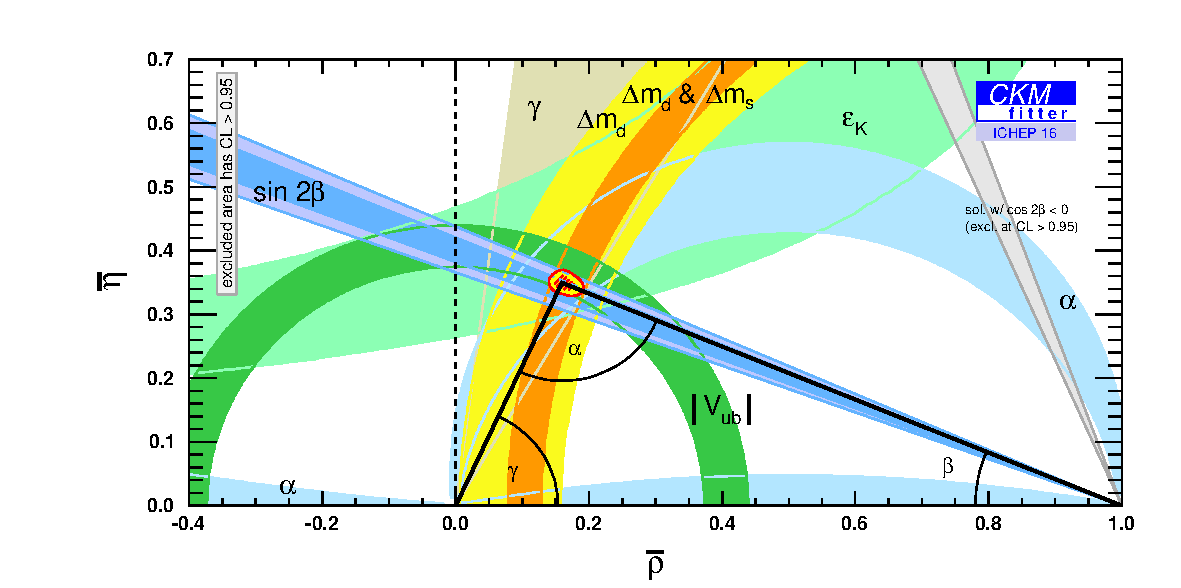
\includegraphics[width=0.7\textwidth]{02theory/figs/ckm_triangle.pdf}
	\caption{$CKM$ triangle in the complexe plane.}
\label{fig:ckmtheory}
\end{figure}
This representation allows a nice experimental tests of the \ac{SM} by overconstraining the triangle with measurements of all three
angles and sides of the triangle.
